\documentclass[a4paper,english]{article}
\usepackage{graphicx}
\usepackage{listings}
%% Use utf-8 encoding for foreign characters
%%\usepackage[T1]{fontenc}
%%\usepackage[utf8]{inputenc}
%%\usepackage{babel}
%%
%%%% Vector based fonts instead of bitmaps
%%\usepackage{lmodern}
%%
%%%% Useful
%%%\usepackage{fullpage} % Smaller margins
%%\usepackage{enumerate}
%%
%%%% Theorem
%%\usepackage{amsthm}
%%
%%%% More math
%%\usepackage{amsmath}
%%\usepackage{amssymb}

%% Document Header
\title{Section2}
\author{Elliott Ashby}
\date{\today}

\begin{document}
    \maketitle
    \section{q1}
        If fabs is ommitted there may arise a situation where total is negative and therefore
        if $1.0e^{-13}$ is added to it would have the opposite effect on the inequality therefore
        not making the desired outcome. Essentially, if term and total are negative, the wrong 
        stopping condition is applied resulting in undesired results. (See Figure 1)
        \begin{figure}
            \caption{Incorrect stopping condition:}
            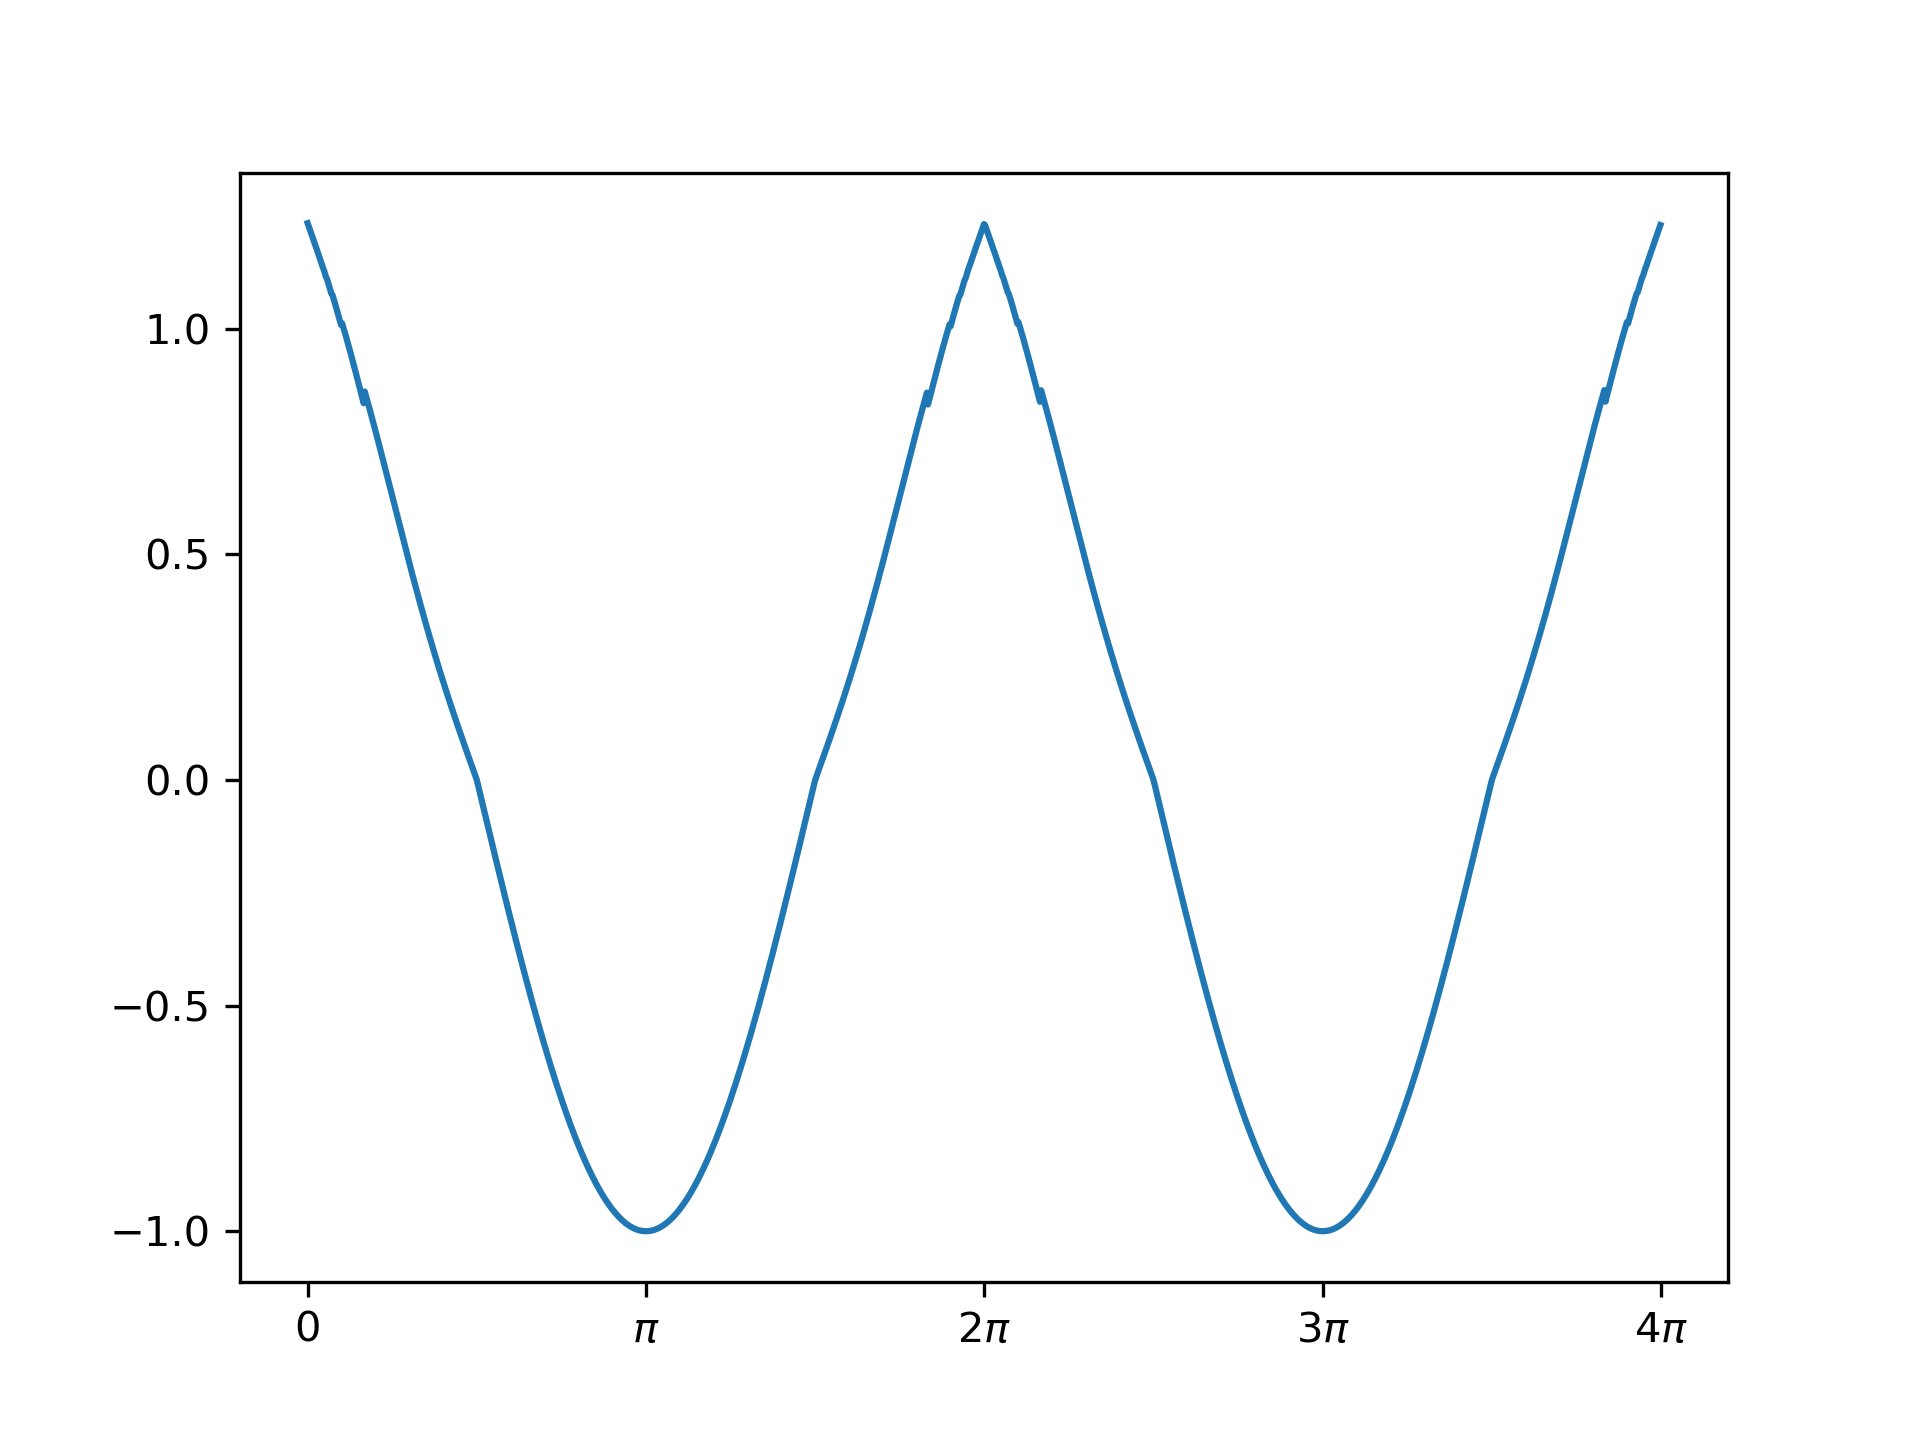
\includegraphics[scale=0.7]{./q1nofabs.png}
        \end{figure}
    \section{q2}
        If $1e^{-26}$ used our relative stopping condition would be more accurate than our absolute one, at $1.0e^{-13}$. The reason, that $1e^{-3}$ isnt used is that, while using a
        less accurate stopping condition is faster, $\pi$ is defined to a much greater degree than 3 decimal places.
    \section{q3}
        \lstinputlisting[language=Python]{./q2_3.py}
        The script here performs the function g(x) over the range 0 to 4$\pi$ and saves it as a graph which can be seen as Figure 2.
        \begin{figure}
            \caption{Correct stopping conditions and correct output of Q2.3:}
            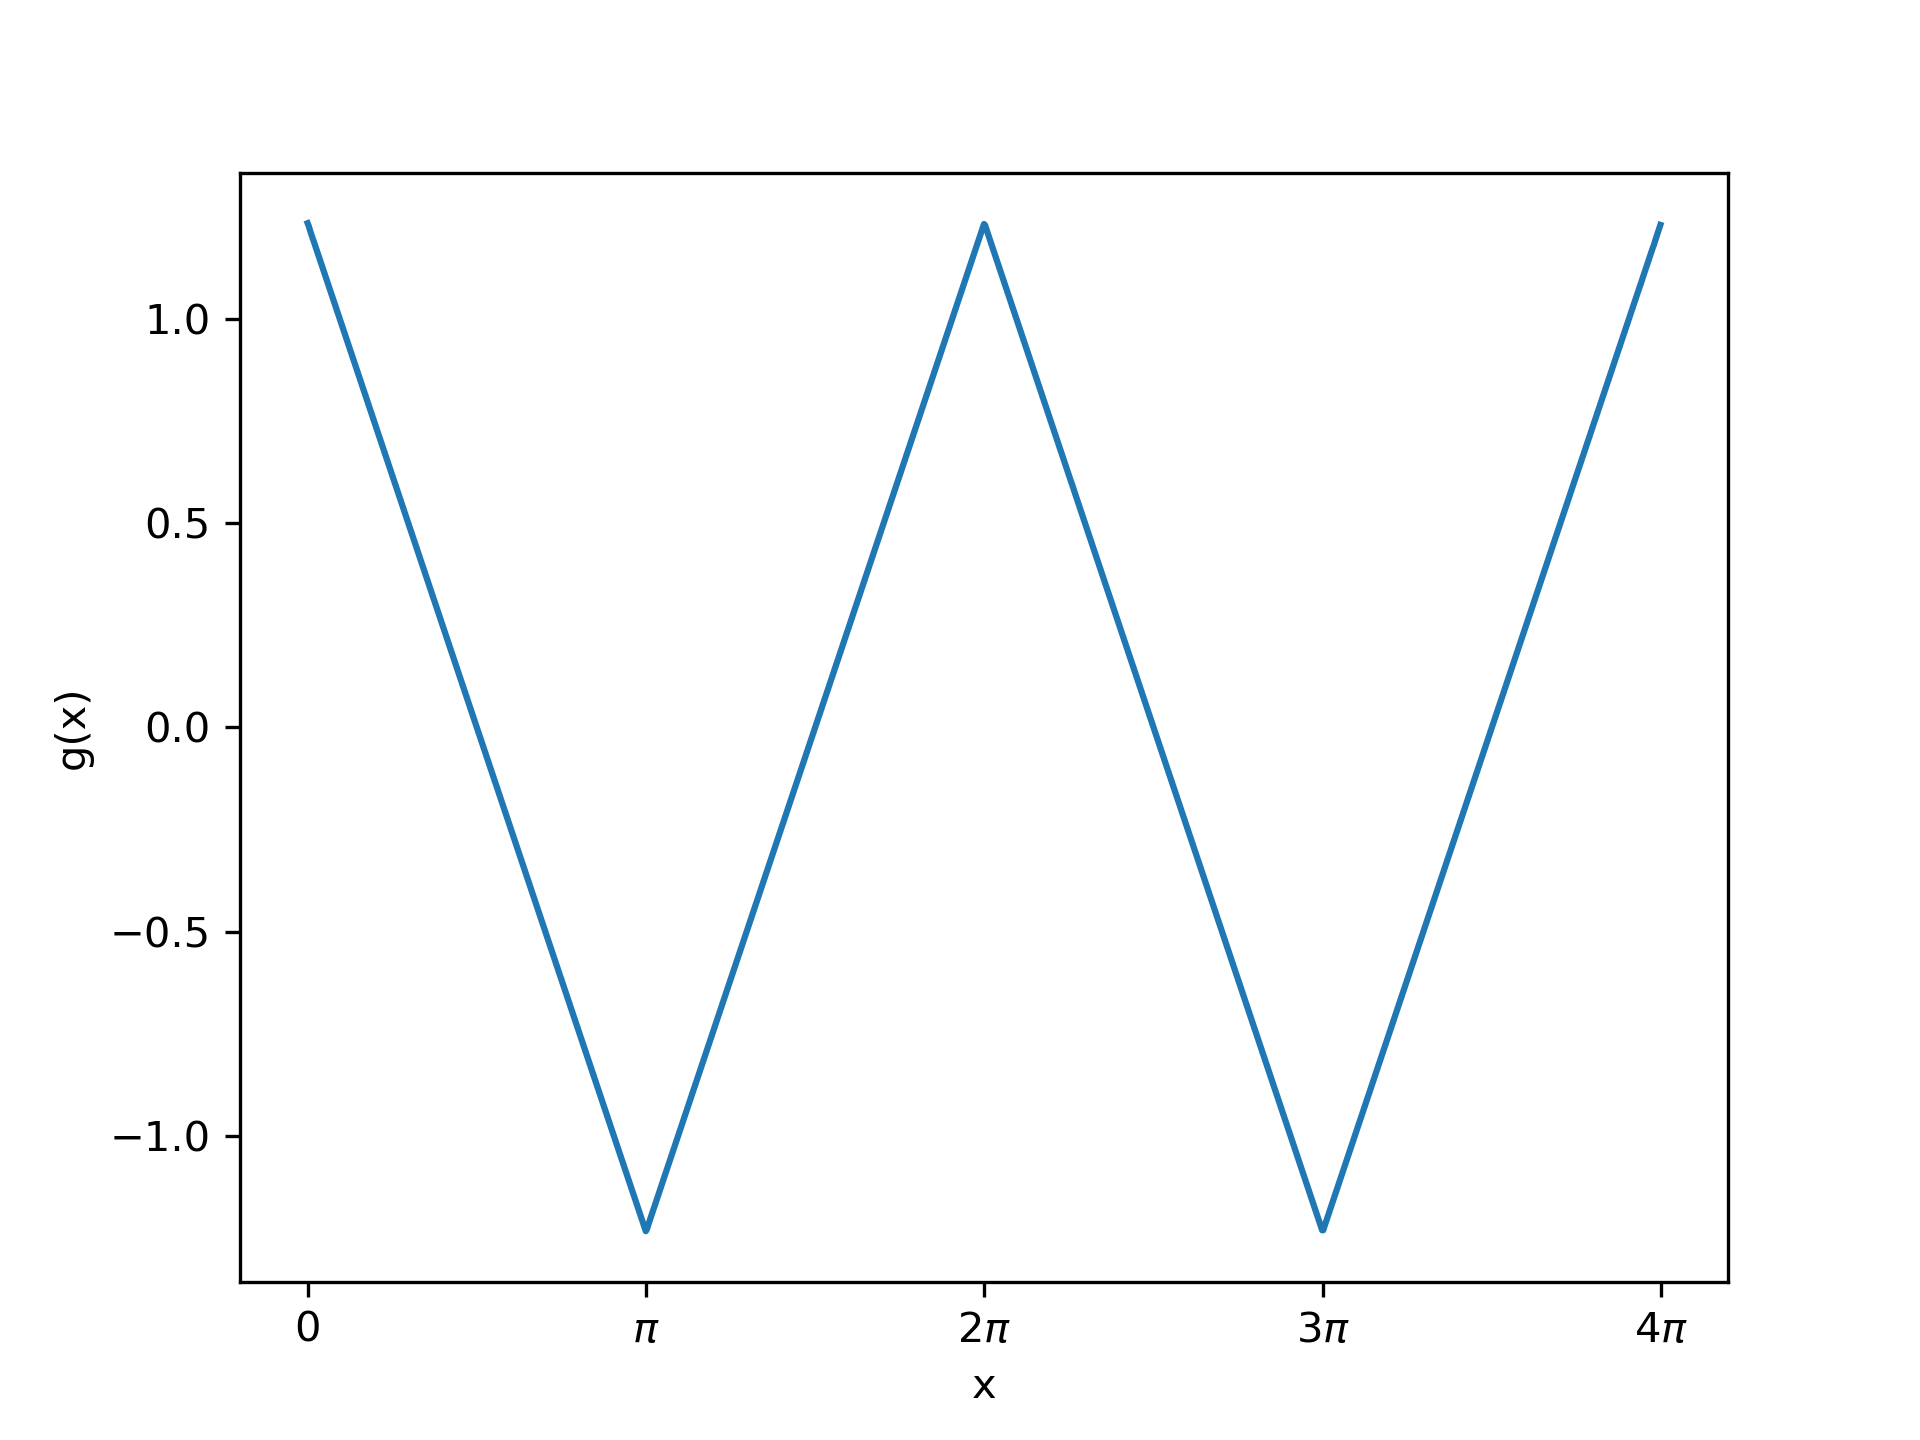
\includegraphics[scale=0.7]{./q2_3.png}
        \end{figure}
    \section{q4}
        \lstinputlisting[language=Python]{./q2_4.py}
        Here, we use a stopping condition to acquire $R_\infty$ and print it. We then generate a list of this approximation as it increases in 
        order to compare the two. The if else statement just allows me to change how many entries b has without needing to worry about the length
        of either list. 
        \\ The script then saves the plot comparing the difference of $R_n$ and $R_\infty$ at different values of $R_n$.
        \begin{figure}
            \caption{$log(R_n - R_\infty$)}
            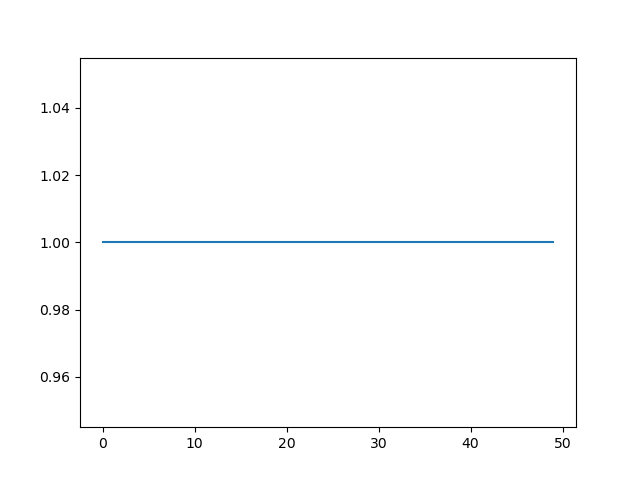
\includegraphics[scale=0.7]{./q2_4.png}
        \end{figure}

    \section{q5}
        $R_n = R_\infty + Ae^{-Bn}$ is a good approximation
        since $R_\infty$ is a constant and as n increases the $Ae^{-Bn}$ term of the right side decreases in size exponentially, meaning 
        that the value of $R_n$ and $R_\infty$ get exponentially closer together until $Ae^{-Bn}$ is negligible at which point $R_n$ and 
        $R_\infty$ are equal (and hence when taken away from one another equate to 0)
\end{document}
